% =====================================================================
% Apresentação - Trabalho de VE - Mecânica II - Grupo I (Pião)
% Compilação: pdflatex apresentacao_grupo_I.tex  (executar 2 vezes)
% Roteiro de fala: compilar apresentacao_grupo_I_notas.tex
% =====================================================================
\documentclass[11pt,aspectratio=169]{beamer}

\usepackage[utf8]{inputenc}
\usepackage[T1]{fontenc}
\usepackage{lmodern}
\usepackage[brazil]{babel}
\usepackage{amsmath,amssymb}
\usepackage{icomma}
\usepackage{graphicx}
\usepackage{booktabs}
\usepackage{appendixnumberbeamer}
\usepackage{tikz}
\usetikzlibrary{arrows.meta,calc}

\graphicspath{{figuras/}}

\definecolor{azul}{HTML}{2A78D6}
\definecolor{azulesc}{HTML}{174A87}
\definecolor{laranja}{HTML}{EB6834}
\definecolor{tinta}{HTML}{1C1C1B}
\definecolor{tinta2}{HTML}{52514E}
\definecolor{apoio}{HTML}{E3E1DA}
\definecolor{corpo}{HTML}{F4E6DC}
\definecolor{corpoesc}{HTML}{DDBBA6}
\definecolor{corpob}{HTML}{A9765A}

\usefonttheme[onlymath]{serif}
\setbeamertemplate{navigation symbols}{}
\setbeamercolor{normal text}{fg=tinta}
\setbeamercolor{frametitle}{fg=azulesc}
\setbeamerfont{frametitle}{series=\bfseries,size=\Large}
\setbeamercolor{itemize item}{fg=azul}
\setbeamercolor{itemize subitem}{fg=azul}
\setbeamercolor{enumerate item}{fg=azulesc}
\setbeamercolor{title}{fg=azulesc}
\setbeamercolor{block title}{fg=white,bg=azulesc}
\setbeamercolor{block body}{fg=tinta,bg=azul!8}
\setbeamertemplate{blocks}[rounded][shadow=false]
\setbeamertemplate{itemize items}[circle]
\setbeamertemplate{footline}{%
  \leavevmode\hbox to \paperwidth{\hspace{0.6cm}\color{tinta2}\scriptsize
    Grupo I -- Pião\hfill\insertframenumber\,/\,\inserttotalframenumber\hspace{0.6cm}}\vspace{0.25cm}}

\ifdefined\SOMENTENOTAS
  \setbeameroption{show only notes}
\fi

% Notação: vetores e tensores em negrito; magnitudes em itálico
\newcommand{\vet}[1]{\mathbf{#1}}
\newcommand{\vomega}{\boldsymbol{\omega}}
\newcommand{\vOmega}{\boldsymbol{\Omega}}
\newcommand{\seno}{\operatorname{sen}}
\newcommand{\un}[1]{\,\mathrm{#1}}
\newcommand{\phid}{\dot{\phi}}
\newcommand{\psid}{\dot{\psi}}
\newcommand{\eps}{\varepsilon}
\newcommand{\figura}[2]{\resizebox{#1}{!}{\begin{minipage}{12.8cm}\input{figuras/#2}\end{minipage}}}

\title{Pião: precessão permanente}
\subtitle{Trabalho de VE -- Mecânica II -- Grupo I}
\institute{Instituto Militar de Engenharia}
\date{9 de novembro de 2026}

\begin{document}

% ---------------------------------------------------------------- 1
\begin{frame}[plain]
  \vspace{0.3cm}
  \begin{center}
    {\small Instituto Militar de Engenharia -- CFG 2.\textsuperscript{o} ano -- Turma A}\\[0.5cm]
    {\usebeamercolor[fg]{title}\huge\bfseries Pião: precessão permanente}\\[0.25cm]
    {\large Trabalho de VE -- Mecânica II -- Grupo I}\\[0.7cm]
    \small
    \begin{tabular}{ll}
      João Eduardo Moro Hoffmann & Lucas Santos Moraes\\
      Maria Eduarda Medina Henriques & Cláudio Erick de Holanda Fontenele\\
      Gabriela de Lima Cardoso & Tiago Alves Porto Lima\\
      Sara Eduarda dos Santos Borges & Marcos Kalile Meira de Vasconcellos
    \end{tabular}\\[0.6cm]
    9 de novembro de 2026
  \end{center}
  \note{[0:00 -- 0:30] Apresentar o grupo e o tema. Dizer em uma frase o objetivo: determinar a que taxas um pião inclinado pode precessar sem mudar de inclinação.}
\end{frame}

% ---------------------------------------------------------------- enunciado
% Salve a imagem do enunciado como figuras/enunciado_grupo_I.png
\begin{frame}[plain]
  \begin{center}
    \IfFileExists{figuras/enunciado_grupo_I.png}{%
      \includegraphics[width=0.78\paperwidth,height=0.92\paperheight,keepaspectratio]{enunciado_grupo_I.png}%
    }{%
      \begin{minipage}{0.85\paperwidth}
        \textbf{GRUPO I}\\[0.2cm]
        \small
        Um pião de 100 g é suportado no ponto fixo $O$. Os raios de giração do pião com respeito a seu eixo de simetria e a seu eixo transversal passando por $O$ são 25 mm e 50 mm, respectivamente. Sabendo que $c=40$ mm e que a taxa de rotação (\textit{spin}) em torno do eixo de simetria é 1800 rpm, determine:\\[0.1cm]
        (a) as possíveis taxas de precessão permanentes para $\theta=30^\circ$ a $60^\circ$;\\
        (b) a condição para a precessão permanente sabendo que $\psid\gg\phid$;\\
        (c) o percentual do erro introduzido quando esta última relação for usada para aproximar a menor das duas taxas de precessão obtida no item (a).
      \end{minipage}%
    }
  \end{center}
  \note{Enunciado do trabalho, lido na íntegra. Destacar as três perguntas: (a) as duas taxas, (b) a condição para spin muito maior que a precessão, (c) o erro dessa aproximação.}
\end{frame}

% ---------------------------------------------------------------- vídeo
% Coloque simulacao_piao.mp4 na mesma pasta do PDF.
% Opcional: figuras/primeiro_quadro.png como miniatura clicável.
\begin{frame}[plain]
  \begin{center}
    {\usebeamercolor[fg]{title}\Large\bfseries Simulação do pião}\\[0.5cm]
    \IfFileExists{firstframe.png}{%
      \href{run:precessao.mp4}{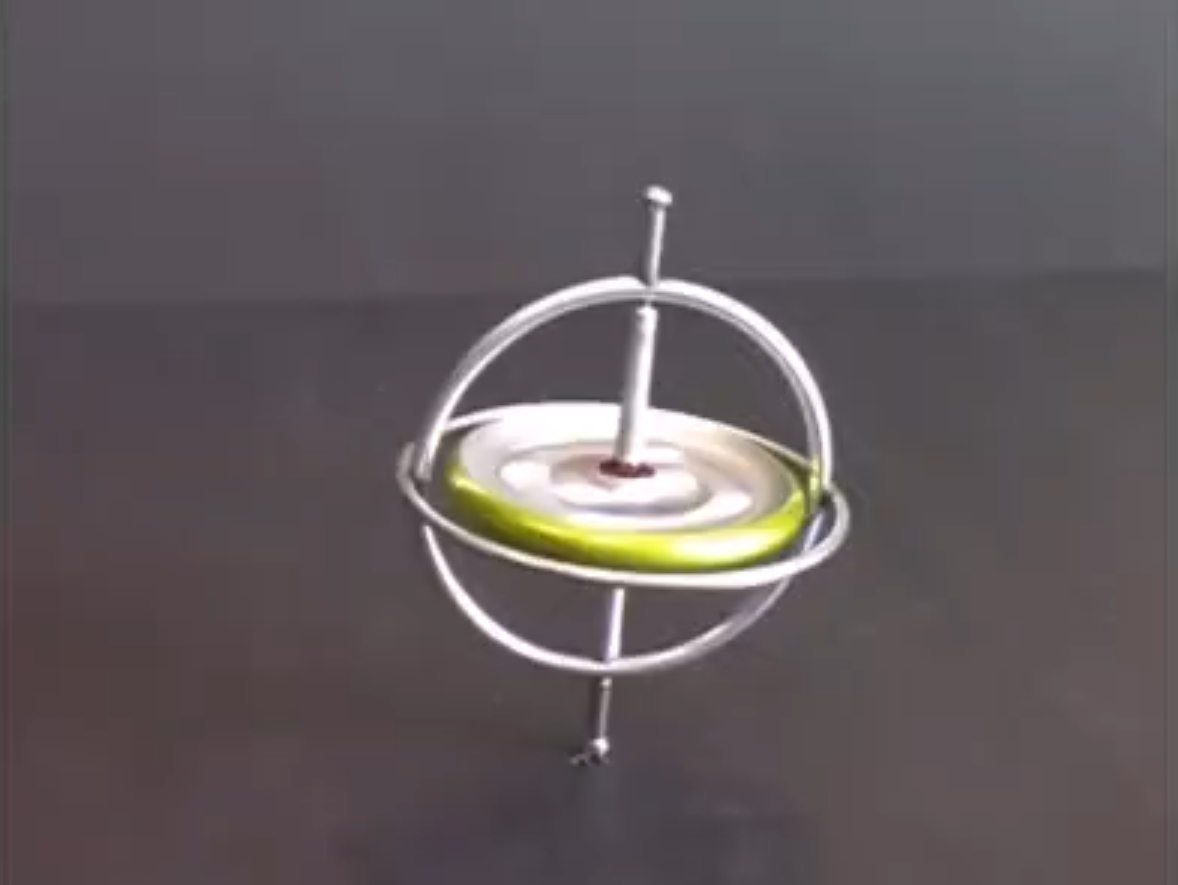
\includegraphics[width=0.6\textwidth]{firstframe.png}}\\[0.3cm]
    }{}%
    {\Large\href{run:precessao.mp4}{\beamerbutton{\textcolor{azulesc}{$\blacktriangleright$ Reproduzir vídeo}}}}
  \end{center}
  \note{Clicar na imagem ou no botão para abrir o vídeo no reprodutor externo. Abrir o vídeo antes da apresentação para conferir se o visualizador permite a execução.}
\end{frame}

% ---------------------------------------------------------------- 2
\begin{frame}{Por que o pião não cai?}
  \begin{columns}[c]
    \begin{column}{0.47\textwidth}
      \begin{itemize}
        \item Parado, ele tomba imediatamente.
        \item Girando, mesmo inclinado, o eixo apenas descreve um cone em torno da vertical: a \textbf{precessão}.
        \item[]
        \item O mesmo princípio governa:
        \begin{itemize}
          \item giroscópios e girobússolas;
          \item projéteis estabilizados por rotação;
          \item orientação de satélites;
          \item precessão do eixo da Terra.
        \end{itemize}
      \end{itemize}
    \end{column}
    \begin{column}{0.48\textwidth}
      \centering
      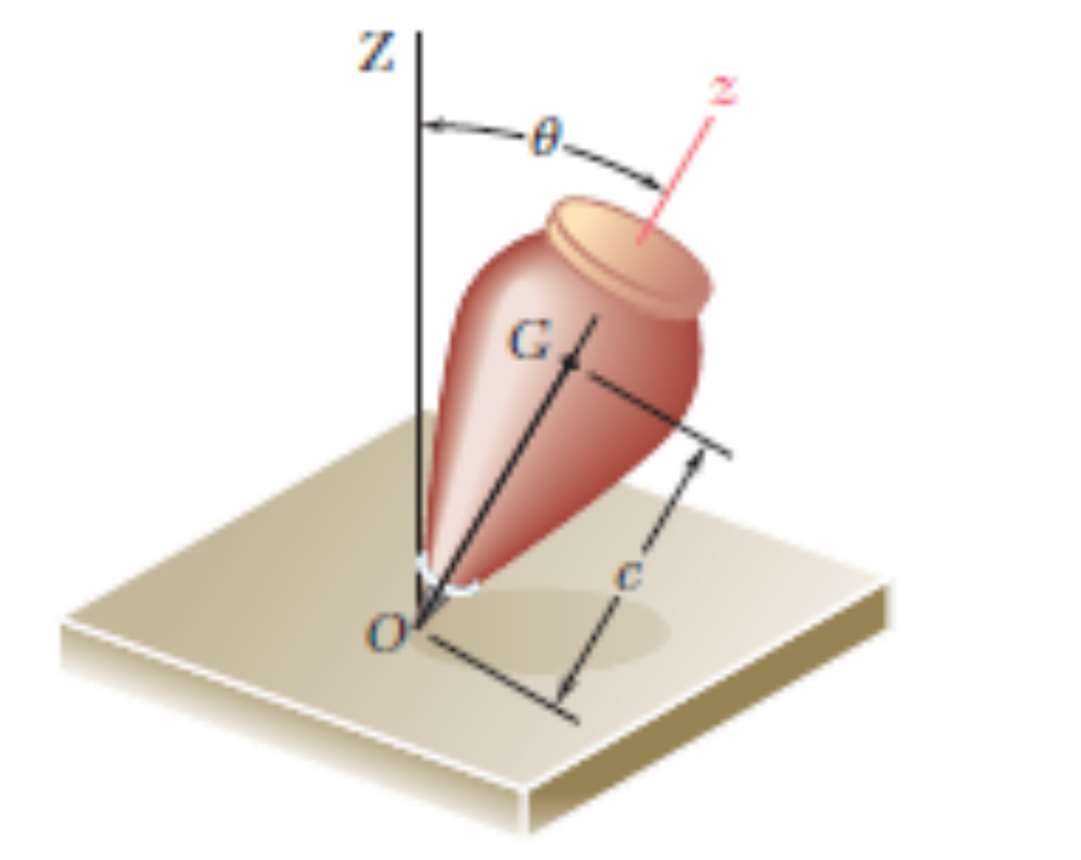
\includegraphics[width=\linewidth]{piao_enunciado.jpg}\\[0.1cm]
      {\scriptsize Figura do enunciado do trabalho.}
    \end{column}
  \end{columns}
  \note{[0:30 -- 1:30] Começar pela pergunta. Se possível, girar um pião real na frente da turma. Ligar o brinquedo às aplicações: o interesse não é o brinquedo, é o princípio dos giroscópios e dos projéteis estabilizados por rotação.}
\end{frame}

% ---------------------------------------------------------------- 3
\begin{frame}{O problema proposto}
  \begin{columns}[t]
    \begin{column}{0.47\textwidth}
      \textbf{Dados}\\[0.2cm]
      \small
      \begin{tabular}{@{}l@{\hspace{0.8em}}l@{}}
        Massa & $m=100\un{g}$\\
        Giração (eixo de simetria) & $k=25\un{mm}$\\
        Giração (transversal por $O$) & $k'=50\un{mm}$\\
        Distância $OG$ & $c=40\un{mm}$\\
        \textit{Spin} & $\psid=1800\un{rpm}$\\
      \end{tabular}\\[0.3cm]
      {\small Adota-se $g=9,81\un{m/s^2}$; corpo rígido, sem atrito, $O$ fixo.}
    \end{column}
    \begin{column}{0.49\textwidth}
      \textbf{Determinar}
      \begin{enumerate}
        \item[(a)] as taxas de precessão permanente possíveis para $\theta=30^\circ$ a $60^\circ$;
        \item[(b)] a condição de precessão permanente quando $\psid\gg\phid$;
        \item[(c)] o erro percentual dessa condição ao aproximar a menor das duas taxas.
      \end{enumerate}
      \vspace{0.3cm}
      \textbf{Precessão permanente:} $\theta$, $\phid$ e $\psid$ constantes.
    \end{column}
  \end{columns}
  \note{[1:30 -- 2:30] Ler os dados e as três perguntas. Definir precessão permanente: a inclinação e as duas taxas não mudam com o tempo. Avisar que g não foi dado e que se adotou 9,81 m/s².}
\end{frame}

% ---------------------------------------------------------------- 4
\begin{frame}{Referencial e forças}
  \begin{center}
    \figura{11.2cm}{diagrama_corpo_livre}
  \end{center}
  \vspace{-0.1cm}
  {\small
  \begin{itemize}
    \item $Oxyz$ acompanha a precessão, não o \textit{spin}; pela simetria, são eixos principais de inércia.
    \item Convenção do livro-texto: $x$ fica abaixo da horizontal e $\vet{j}=\vet{k}\times\vet{i}$ entra no plano em (b).
  \end{itemize}}
  \note{[2:30 -- 3:30] Em (a): Z é fixo, z é o eixo de simetria, x está no plano Zz, y é perpendicular. Explicar a escolha: o referencial gira com a precessão, então H tem componentes constantes nele. Em (b): a reação em O não dá momento em relação a O; por isso O é o ponto de referência. Só o peso produz momento. Se perguntarem por que x aponta para baixo: é consequência de K = -sen(theta) i + cos(theta) k, a convenção do Beer; os eixos são geométricos, não partes do pião.}
\end{frame}

% ---------------------------------------------------------------- 5
\begin{frame}{Cinemática e quantidade de movimento angular}
  \begin{columns}[c]
    \begin{column}{0.6\textwidth}
      \figura{\linewidth}{diagrama_vetores}
    \end{column}
    \begin{column}{0.38\textwidth}
      \small
      \begin{align*}
        \vomega &= \phid\,\vet{K}+\psid\,\vet{k}\\
                &= -\phid\seno\theta\,\vet{i}+\omega_z\,\vet{k}\\[0.1cm]
        \omega_z &= \psid+\phid\cos\theta\\[0.1cm]
        \vet{H}_O &= -I'\phid\seno\theta\,\vet{i}+I\omega_z\,\vet{k}\\[0.2cm]
        I &= mk^2\\
          &= 6,25\times10^{-5}\un{kg\cdot m^2}\\
        I' &= mk'^2\\
           &= 2,50\times10^{-4}\un{kg\cdot m^2}
      \end{align*}
    \end{column}
  \end{columns}
  \vspace{0.1cm}
  \begin{center}
    \small Todos no plano $Zz$; $\vet{H}_O$ \textbf{não} é paralelo a $\vomega$ nem ao eixo de simetria.
  \end{center}
  \note{[3:30 -- 4:30] A velocidade angular é a soma da precessão em torno de Z com o spin em torno de z. Projetar em i e k. Como os eixos são principais, cada componente de H é o momento de inércia vezes a componente de omega. Destacar que omega e H não são paralelos, pois I é diferente de I'.}
\end{frame}

% ---------------------------------------------------------------- 6
\begin{frame}{O princípio: o peso faz $\vet{H}_O$ girar}
  \begin{columns}[c]
    \begin{column}{0.56\textwidth}
      Na precessão permanente, $\vet{H}_O$ é constante em $Oxyz$:
      \[
        \sum\vet{M}_O=\underbrace{\left(\dot{\vet{H}}_O\right)_{Oxyz}}_{=\,\vet{0}}+\vOmega\times\vet{H}_O
        =\vOmega\times\vet{H}_O
      \]
      com $\vOmega=\phid\,\vet{K}$.\\[0.2cm]
      Os dois lados da equação:
      \begin{align*}
        \vOmega\times\vet{H}_O &= \left(I\omega_z-I'\phid\cos\theta\right)\phid\seno\theta\,\vet{j}\\
        \vet{r}_G\times\vet{W} &= Wc\seno\theta\,\vet{j}
      \end{align*}
    \end{column}
    \begin{column}{0.4\textwidth}
      \begin{block}{Interpretação}
        O momento do peso aponta segundo $\vet{j}$, \textbf{perpendicular} ao plano $Zz$.\\[0.15cm]
        Por isso o eixo se desloca para o lado, em vez de tombar.
      \end{block}
    \end{column}
  \end{columns}
  \note{[4:30 -- 6:00] Este é o slide mais importante. A derivada de H tem duas partes: a variação medida em Oxyz, nula, e a causada pela rotação do referencial. Logo, o momento externo só faz o vetor H girar em torno da vertical, sem mudar de intensidade. O momento do peso é horizontal e perpendicular ao plano Zz, e essa é a resposta à pergunta inicial. O produto vetorial é aberto no próximo slide.}
\end{frame}

% ---------------------------------------------------------------- 7
\begin{frame}{Os dois lados, passo a passo}
  \small
  \textbf{Lado da quantidade de movimento}, com $\vOmega=-\phid\seno\theta\,\vet{i}+\phid\cos\theta\,\vet{k}$:
  \[
    \vOmega\times\vet{H}_O=
    \begin{vmatrix}
      \vet{i}&\vet{j}&\vet{k}\\
      -\phid\seno\theta&0&\phid\cos\theta\\
      -I'\phid\seno\theta&0&I\omega_z
    \end{vmatrix}
    =\left(I\omega_z-I'\phid\cos\theta\right)\phid\seno\theta\,\vet{j}
  \]
  A coluna central nula elimina as componentes $\vet{i}$ e $\vet{k}$: só resta $\vet{j}$.\\[0.25cm]
  \textbf{Lado do peso}, com $\vet{K}=-\seno\theta\,\vet{i}+\cos\theta\,\vet{k}$ e $\vet{k}\times\vet{i}=\vet{j}$:
  \[
    \vet{r}_G\times\vet{W}
    =c\,\vet{k}\times\left(W\seno\theta\,\vet{i}-W\cos\theta\,\vet{k}\right)
    =Wc\seno\theta\,\vet{j}
  \]
  \begin{center}
    Os dois lados têm a direção de $\vet{j}$: basta igualar os coeficientes.
  \end{center}
  \note{[6:00 -- 7:00] Mostrar que só a componente j sobrevive. No determinante, a coluna do meio é zero, então i e k se anulam. No peso, k vezes k é zero e k vezes i é j. As contas completas estão no memorial de cálculo.}
\end{frame}

% ---------------------------------------------------------------- 8
\begin{frame}{Equação da precessão permanente}
  Igualando os lados e dividindo por $\seno\theta\neq0$; depois, $\omega_z=\psid+\phid\cos\theta$:
  \begin{align*}
    \phid\left[I\left(\psid+\phid\cos\theta\right)-I'\phid\cos\theta\right]&=Wc\\
    I\psid\,\phid+I\cos\theta\,\phid^{\,2}-I'\cos\theta\,\phid^{\,2}&=Wc
  \end{align*}
  \begin{block}{Equação geral (segundo grau em $\phid$)}
    \[
      (I'-I)\cos\theta\;\phid^{\,2}-I\psid\,\phid+Wc=0
    \]
  \end{block}
  \vspace{0.15cm}
  Como $I=mk^2$, $I'=mk'^2$ e $W=mg$, divide-se por $m$:
  \[
    (k'^2-k^2)\cos\theta\;\phid^{\,2}-k^2\psid\,\phid+gc=0
  \]
  \begin{center}
    \textbf{A massa se cancela:} as taxas dependem só da geometria e de $g$.
  \end{center}
  \note{[7:00 -- 8:00] Fazer a distributiva e agrupar os termos em phi ao quadrado. Duas raízes significam dois movimentos possíveis para o mesmo spin e a mesma inclinação. Comentar que a massa se cancela: um pião geometricamente igual, porém mais pesado, precessa à mesma taxa.}
\end{frame}

% ---------------------------------------------------------------- 8
\begin{frame}{Item (a): cálculo para $\theta=30^\circ$}
  \begin{columns}[c]
    \begin{column}{0.54\textwidth}
      Com $a=(I'-I)\cos\theta$ e $b=I\psid$:
      \[
        \phid_{1,2}=\frac{b\mp\sqrt{b^2-4aWc}}{2a}
      \]
      \begin{align*}
        a &= 1,6238\times10^{-4}\un{kg\cdot m^2}\\
        b &= 0,011781\un{kg\cdot m^2/s}\\
        Wc &= 0,03924\un{N\cdot m}\\
        b^2 &= 1,3879\times10^{-4}\\
        4aWc &= 0,2549\times10^{-4}\\
        \sqrt{b^2-4aWc} &= \sqrt{1,1330\times10^{-4}}=0,010644
      \end{align*}
    \end{column}
    \begin{column}{0.42\textwidth}
      \begin{block}{Resultado para $\theta=30^\circ$}
        \begin{align*}
          \phid_1 &= 3,50\un{rad/s}=33,4\un{rpm}\\
          \phid_2 &= 69,05\un{rad/s}=659\un{rpm}
        \end{align*}
      \end{block}
      \vspace{0.2cm}
      {\small Verificação: $\phid_1\phid_2=Wc/a=241,7\un{rad^2/s^2}$.\\[0.1cm]
      As duas raízes são positivas: ambas têm o sentido do \textit{spin}.}
    \end{column}
  \end{columns}
  \note{[8:00 -- 9:30] Fazer a conta com calma. O spin de 1800 rpm equivale a 188,50 rad/s. Mencionar a verificação pelo produto das raízes. Chamar phi1 de precessão lenta e phi2 de rápida.}
\end{frame}

% ---------------------------------------------------------------- 9
\begin{frame}{Item (a): toda a faixa de inclinação}
  \begin{columns}[c]
    \begin{column}{0.3\textwidth}
      \centering\small
      \begin{tabular}{ccc}
        \toprule
        $\theta$ & $\phid_1$ & $\phid_2$\\
         & (rad/s) & (rad/s)\\
        \midrule
        $30^\circ$ & $3,500$ & $69,05$\\
        $35^\circ$ & $3,490$ & $73,21$\\
        $40^\circ$ & $3,478$ & $78,54$\\
        $45^\circ$ & $3,466$ & $85,39$\\
        $50^\circ$ & $3,453$ & $94,30$\\
        $55^\circ$ & $3,439$ & $106,11$\\
        $60^\circ$ & $3,424$ & $122,24$\\
        \bottomrule
      \end{tabular}
    \end{column}
    \begin{column}{0.67\textwidth}
      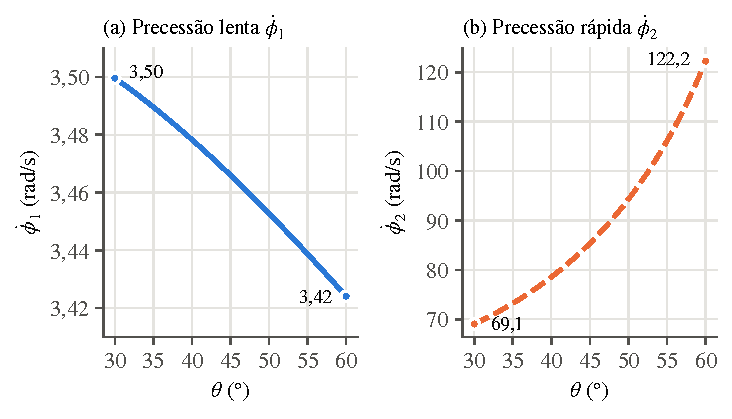
\includegraphics[width=\linewidth]{taxas_precessao_slide.pdf}
    \end{column}
  \end{columns}
  \vspace{0.2cm}
  \begin{center}
    A lenta quase não muda ($-2,2\%$); a rápida cresce $77\%$.\\
    {\small Atenção: as escalas verticais dos gráficos são diferentes.}
  \end{center}
  \note{[9:30 -- 11:00] Comparar os dois gráficos, avisando que as escalas diferem. A lenta é quase independente de theta, o que antecipa o item (b). Fim da primeira parte: o segundo apresentador assume a partir daqui.}
\end{frame}

% ---------------------------------------------------------------- 10
\begin{frame}{Item (b): condição para $\psid\gg\phid$}
  A equação geral pode ser escrita como $\phid\,(b-a\phid)=Wc$, com $a=(I'-I)\cos\theta$ e $b=I\psid$.\\[0.1cm]
  Se $\psid\gg\phid$, despreza-se $a\phid$ diante de $b$:
  \begin{block}{Condição de precessão permanente}
    \[
      \phid_a\approx\frac{Wc}{I\psid}=\frac{mgc}{I\psid}=\frac{0,03924}{0,011781}=3,33\un{rad/s}=31,8\un{rpm}
    \]
  \end{block}
  \vspace{0.2cm}
  \begin{itemize}
    \item Equivale a admitir $\vet{H}_O\approx I\psid\,\vet{k}$: então $Wc\seno\theta=\phid\,I\psid\seno\theta$.
    \item O fator $\seno\theta$ se cancela: a taxa \textbf{independe da inclinação}.
    \item Quanto \textbf{mais rápido} o \textit{spin}, \textbf{mais lenta} a precessão.
    \item Vale só para a raiz lenta: na rápida, $\phid_2/\psid$ vai de $0,37$ a $0,65$.
  \end{itemize}
  \note{[11:00 -- 12:30] Esta é a resposta do item (b). Em 30 graus, o termo desprezado é 4,8\% de b. Interpretar: H fica praticamente alinhado com o eixo de simetria. Explicar por que o resultado não depende de theta. Ressaltar que a hipótese não se aplica à raiz rápida, pois ela não é pequena diante do spin.}
\end{frame}

% ---------------------------------------------------------------- 11
\begin{frame}{Item (c): erro da aproximação}
  \begin{columns}[c]
    \begin{column}{0.36\textwidth}
      \[
        e=\frac{\phid_a-\phid_1}{\phid_1}\times100\%
      \]
      \[
        e_{30^\circ}=\frac{3,331-3,500}{3,500}\times100\%
      \]
      \begin{block}{Resultado}
        \centering
        $e=-4,82\%$ em $\theta=30^\circ$\\
        $e=-2,72\%$ em $\theta=60^\circ$
      \end{block}
      \vspace{0.1cm}
      {\small O sinal negativo indica que a aproximação subestima a taxa exata.}
    \end{column}
    \begin{column}{0.62\textwidth}
      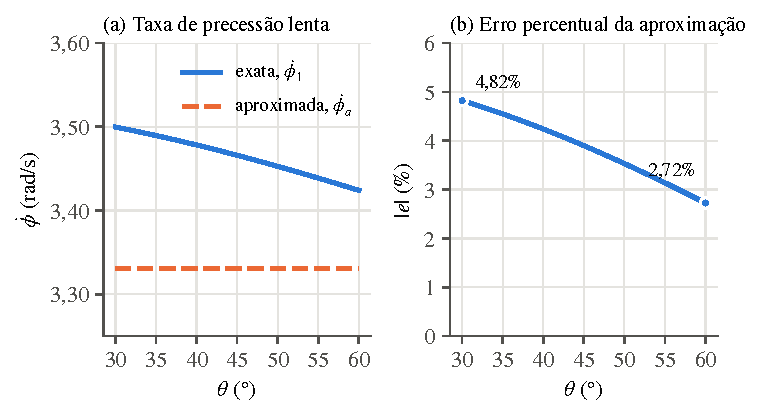
\includegraphics[width=\linewidth]{erro_aproximacao_slide.pdf}
    \end{column}
  \end{columns}
  \note{[12:30 -- 13:30] A aproximação é constante, 3,33 rad/s, enquanto a taxa exata varia pouco. O erro é pequeno para uma estimativa de engenharia. O próximo slide mostra de onde ele vem.}
\end{frame}

% ---------------------------------------------------------------- 13
\begin{frame}{Item (c): de onde vem o erro}
  \begin{columns}[c]
    \begin{column}{0.54\textwidth}
      $\phid_1$ é raiz de $\phid\,(b-a\phid)=Wc$. Dividindo por $b\,\phid_1$:
      \[
        1-\frac{a\phid_1}{b}=\frac{Wc}{b\,\phid_1}=\frac{\phid_a}{\phid_1}
      \]
      Como $e/100\%=\phid_a/\phid_1-1$:
      \[
        \frac{e}{100\%}=-\frac{a\phid_1}{b}
      \]
      Substituindo a raiz $\phid_1$, com $\eps=aWc/b^2$:
      \[
        \frac{e}{100\%}=\frac{\sqrt{1-4\eps}-1}{2}\approx-\eps
      \]
    \end{column}
    \begin{column}{0.42\textwidth}
      \begin{block}{Interpretação}
        O erro é exatamente a razão entre o termo \textbf{desprezado} e o termo \textbf{mantido}.
      \end{block}
      \vspace{0.2cm}
      {\small
      Em $\theta=30^\circ$: $\eps=0,0459$, $e=-4,82\%$ (exato) e $-4,59\%$ (só com $-\eps$).\\[0.15cm]
      Como $\eps\propto1/\psid^{\,2}$, dobrar o \textit{spin} reduz o erro a cerca de um quarto.}
    \end{column}
  \end{columns}
  \note{[13:30 -- 15:00] Partir da equação do item (b) sem desprezar nada. A conta mostra que o erro não é um número solto: é o termo que foi jogado fora, dividido pelo que ficou. A expressão em epsilon deixa claro que o erro cai com o quadrado do spin, e isso é o que o próximo slide mostra.}
\end{frame}

% ---------------------------------------------------------------- 12
\begin{frame}{Aprofundamento: influência do \textit{spin}}
  \begin{center}
    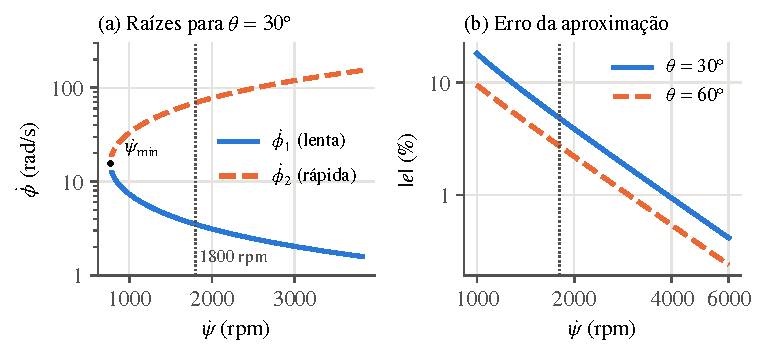
\includegraphics[width=0.64\linewidth]{efeito_spin_slide.pdf}
  \end{center}
  \begin{itemize}
    \item Existe um \textit{spin} mínimo: $\displaystyle\psid_{\mathrm{min}}=\frac{2}{I}\sqrt{(I'-I)\cos\theta\;Wc}$, igual a $771\un{rpm}$ em $\theta=30^\circ$.
    \item O erro decai aproximadamente com $1/\psid^{\,2}$; fica abaixo de $1\%$ perto de $4000\un{rpm}$ em $\theta=30^\circ$.
  \end{itemize}
  \note{[15:00 -- 16:00] Painel (a): abaixo do spin mínimo, a equação não tem raízes reais e não há precessão permanente; acima dele, as raízes se afastam. A linha pontilhada marca os 1800 rpm do problema. Painel (b): em escala logarítmica, a reta mostra o decaimento do erro.}
\end{frame}

% ---------------------------------------------------------------- 13
\begin{frame}{Por que só se observa a precessão lenta?}
  \begin{columns}[c]
    \begin{column}{0.56\textwidth}
      \centering\small
      \begin{tabular}{ccccc}
        \toprule
        $\theta$ & Solução & $\phid/\psid$ & $E$ (J) & $R_h/W$\\
        \midrule
        $30^\circ$ & lenta & $0,019$ & $1,181$ & $0,025$\\
                   & rápida & $0,366$ & $2,110$ & $9,72$\\
        $45^\circ$ & lenta & $0,018$ & $1,168$ & $0,035$\\
                   & rápida & $0,453$ & $2,419$ & $21,0$\\
        $60^\circ$ & lenta & $0,018$ & $1,151$ & $0,041$\\
                   & rápida & $0,649$ & $3,368$ & $52,8$\\
        \bottomrule
      \end{tabular}\\[0.3cm]
      $R_h=mc\seno\theta\;\phid^{\,2}$ \quad (força centrípeta de $G$)
    \end{column}
    \begin{column}{0.4\textwidth}
      \begin{itemize}
        \item \textbf{Lenta:} força horizontal de até $4,1\%$ do peso; um atrito modesto a sustenta.
        \item \textbf{Rápida:} de $9,7$ a $53$ vezes o peso; a ponta deslizaria em um plano comum.
        \item A rápida exige ainda de $1,8$ a $2,9$ vezes mais energia.
      \end{itemize}
    \end{column}
  \end{columns}
  \note{[16:00 -- 17:30] As duas soluções são matematicamente válidas. A rápida só é viável com O realmente fixo, como admite o enunciado. Observação: o atrito é desprezado como dissipação e momento, mas a força horizontal em O é uma reação necessária, pois G descreve uma circunferência.}
\end{frame}

% ---------------------------------------------------------------- 15
\begin{frame}{Validação numérica independente}
  \begin{columns}[c]
    \begin{column}{0.62\textwidth}
      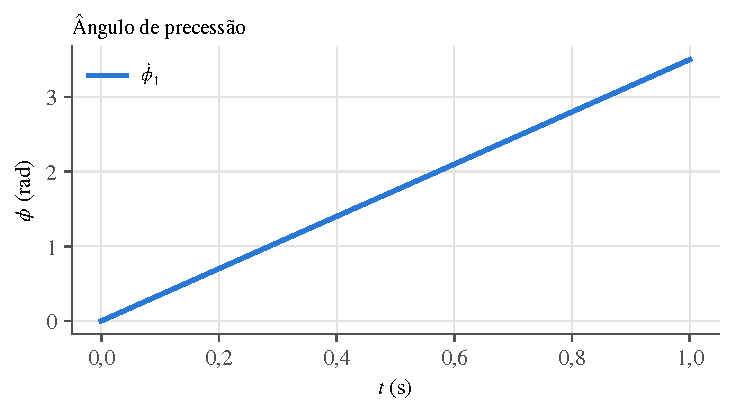
\includegraphics[width=\linewidth]{simulacao_slide.pdf}
    \end{column}
    \begin{column}{0.35\textwidth}
      {\small
      \textbf{Método:} equações de Euler em eixos do corpo, quatérnios e Runge--Kutta de 4.ª ordem.\\[0.2cm]
      \textbf{Independência:} não usa a equação de segundo grau.\\[0.2cm]
      \textbf{Taxas:} desvio $<10^{-8}\%$ em relação às raízes.\\[0.2cm]
      \textbf{Inclinação:} $\theta$ constante, com variação $<10^{-8}$ graus.}
    \end{column}
  \end{columns}
  \note{[17:30 -- 18:15] A simulação não usa a equação de segundo grau nem os ângulos de Euler; por isso é uma verificação independente. A reta mostra phi crescendo a taxa constante, com theta constante: é a precessão permanente prevista.}
\end{frame}

% ---------------------------------------------------------------- 16
\begin{frame}{Conclusão}
  \begin{itemize}
    \item O momento do peso faz $\vet{H}_O$ \textbf{girar}, em vez de derrubar o pião; a resposta não depende da massa.
    \item \textbf{(a)} Duas taxas: lenta de $3,50$ a $3,42\un{rad/s}$ e rápida de $69,1$ a $122,2\un{rad/s}$.
    \item \textbf{(b)} Para $\psid\gg\phid$: $\phid_a\approx Wc/(I\psid)=3,33\un{rad/s}$, independente de $\theta$.
    \item \textbf{(c)} Erro de $4,82\%$ a $2,72\%$, sempre por falta.
    \item As duas soluções existem acima de um \textit{spin} mínimo, mas só a lenta é fisicamente acessível a um pião comum.
    \item A integração numérica independente confirmou os resultados.
  \end{itemize}
  \vspace{0.3cm}
  {\small\textbf{Limitações do modelo:} não representa o decaimento do \textit{spin} por atrito nem o deslizamento da ponta.}
  \note{[18:15 -- 19:15] Retomar a pergunta inicial: o pião não cai porque o momento do peso é perpendicular ao plano de queda. Dar as três respostas e citar as limitações. Sobra cerca de 1 minuto de margem.}
\end{frame}

% ---------------------------------------------------------------- 17
\begin{frame}[plain]
  \begin{center}
    {\usebeamercolor[fg]{title}\Huge\bfseries Perguntas?}\\[0.8cm]
    {\small BEER, F. P.; JOHNSTON JR., E. R.; CORNWELL, P. J. \textit{Mecânica Vetorial para Engenheiros: Dinâmica}. 9. ed. Porto Alegre: AMGH, 2012.}
  \end{center}
  \note{Arguição: cerca de 5 minutos. Os slides seguintes são de apoio; use-os apenas se surgirem perguntas sobre esses pontos.}
\end{frame}

\appendix

% ---------------------------------------------------------------- apoio
\begin{frame}{Apoio: casos particulares}
  \begin{block}{Inclinação acima de $90^\circ$}
    Como $\phid_1\phid_2=Wc/a$ e $a<0$, as raízes têm sinais opostos: uma das precessões passa a ter sentido contrário ao do \textit{spin}.
  \end{block}
  \vspace{0.2cm}
  \begin{block}{Massa}
    A massa se cancela nas taxas e em $R_h/W=c\seno\theta\,\phid^{\,2}/g$.
  \end{block}
  \note{Usar se perguntarem sobre inclinações maiores ou sobre o efeito da massa.}
\end{frame}

\end{document}
'